\chapter*{Extra figures}
\label{ch:extra_figures}
\addcontentsline{toc}{chapter}{Extra figures}

To make the report more readable some figures are not provided directly in the text.
These figures are provided here.

\section*{Login required page}

\begin{figure}[H]
    \centering
    \includegraphics[width=\linewidth]{images/loginrequired.png}
    \captionsetup{width=0.9\linewidth}
    \captionsetup{justification=centering}
    \caption{Page notifying the user an account is required.}
    \label{fig:login-requred}
\end{figure}

\clearpage
\section*{Register and login page}

\begin{figure}[H]
     \centering
     \begin{subfigure}[b]{0.9\textwidth}
         \centering
         \includegraphics[width=\textwidth]{images/register.png}
         \caption{Register page with validation that username is already in use.}
         \label{fig:register}
     \end{subfigure}
     \hfill
     \begin{subfigure}[b]{0.9\textwidth}
         \centering
         \includegraphics[width=\textwidth]{images/login.png}
         \caption{Login page with flash message.}
         \label{fig:login}
     \end{subfigure}
        \caption{Login and register page of CarLovers website.}
        \label{fig:login_register}
\end{figure}


\section*{Overview and profile page}

\begin{figure}[H]
     \centering
     \begin{subfigure}[b]{0.9\textwidth}
         \centering
         \includegraphics[width=\textwidth]{images/homesnellen.png}
         \caption{The main overview page which may be sorted on date or likes.}
         \label{fig:overview}
     \end{subfigure}
     \hfill
     \begin{subfigure}[b]{0.9\textwidth}
         \centering
         \includegraphics[width=\textwidth]{images/profile.png}
         \caption{The profile page of a specific user.}
         \label{fig:profile}
     \end{subfigure}
        \caption{Overview and profile page of Carlovers that share sub-views.}
        \label{fig:overview_profile}
\end{figure}


\section*{Single post page}

\begin{figure}[H]
    \centering
    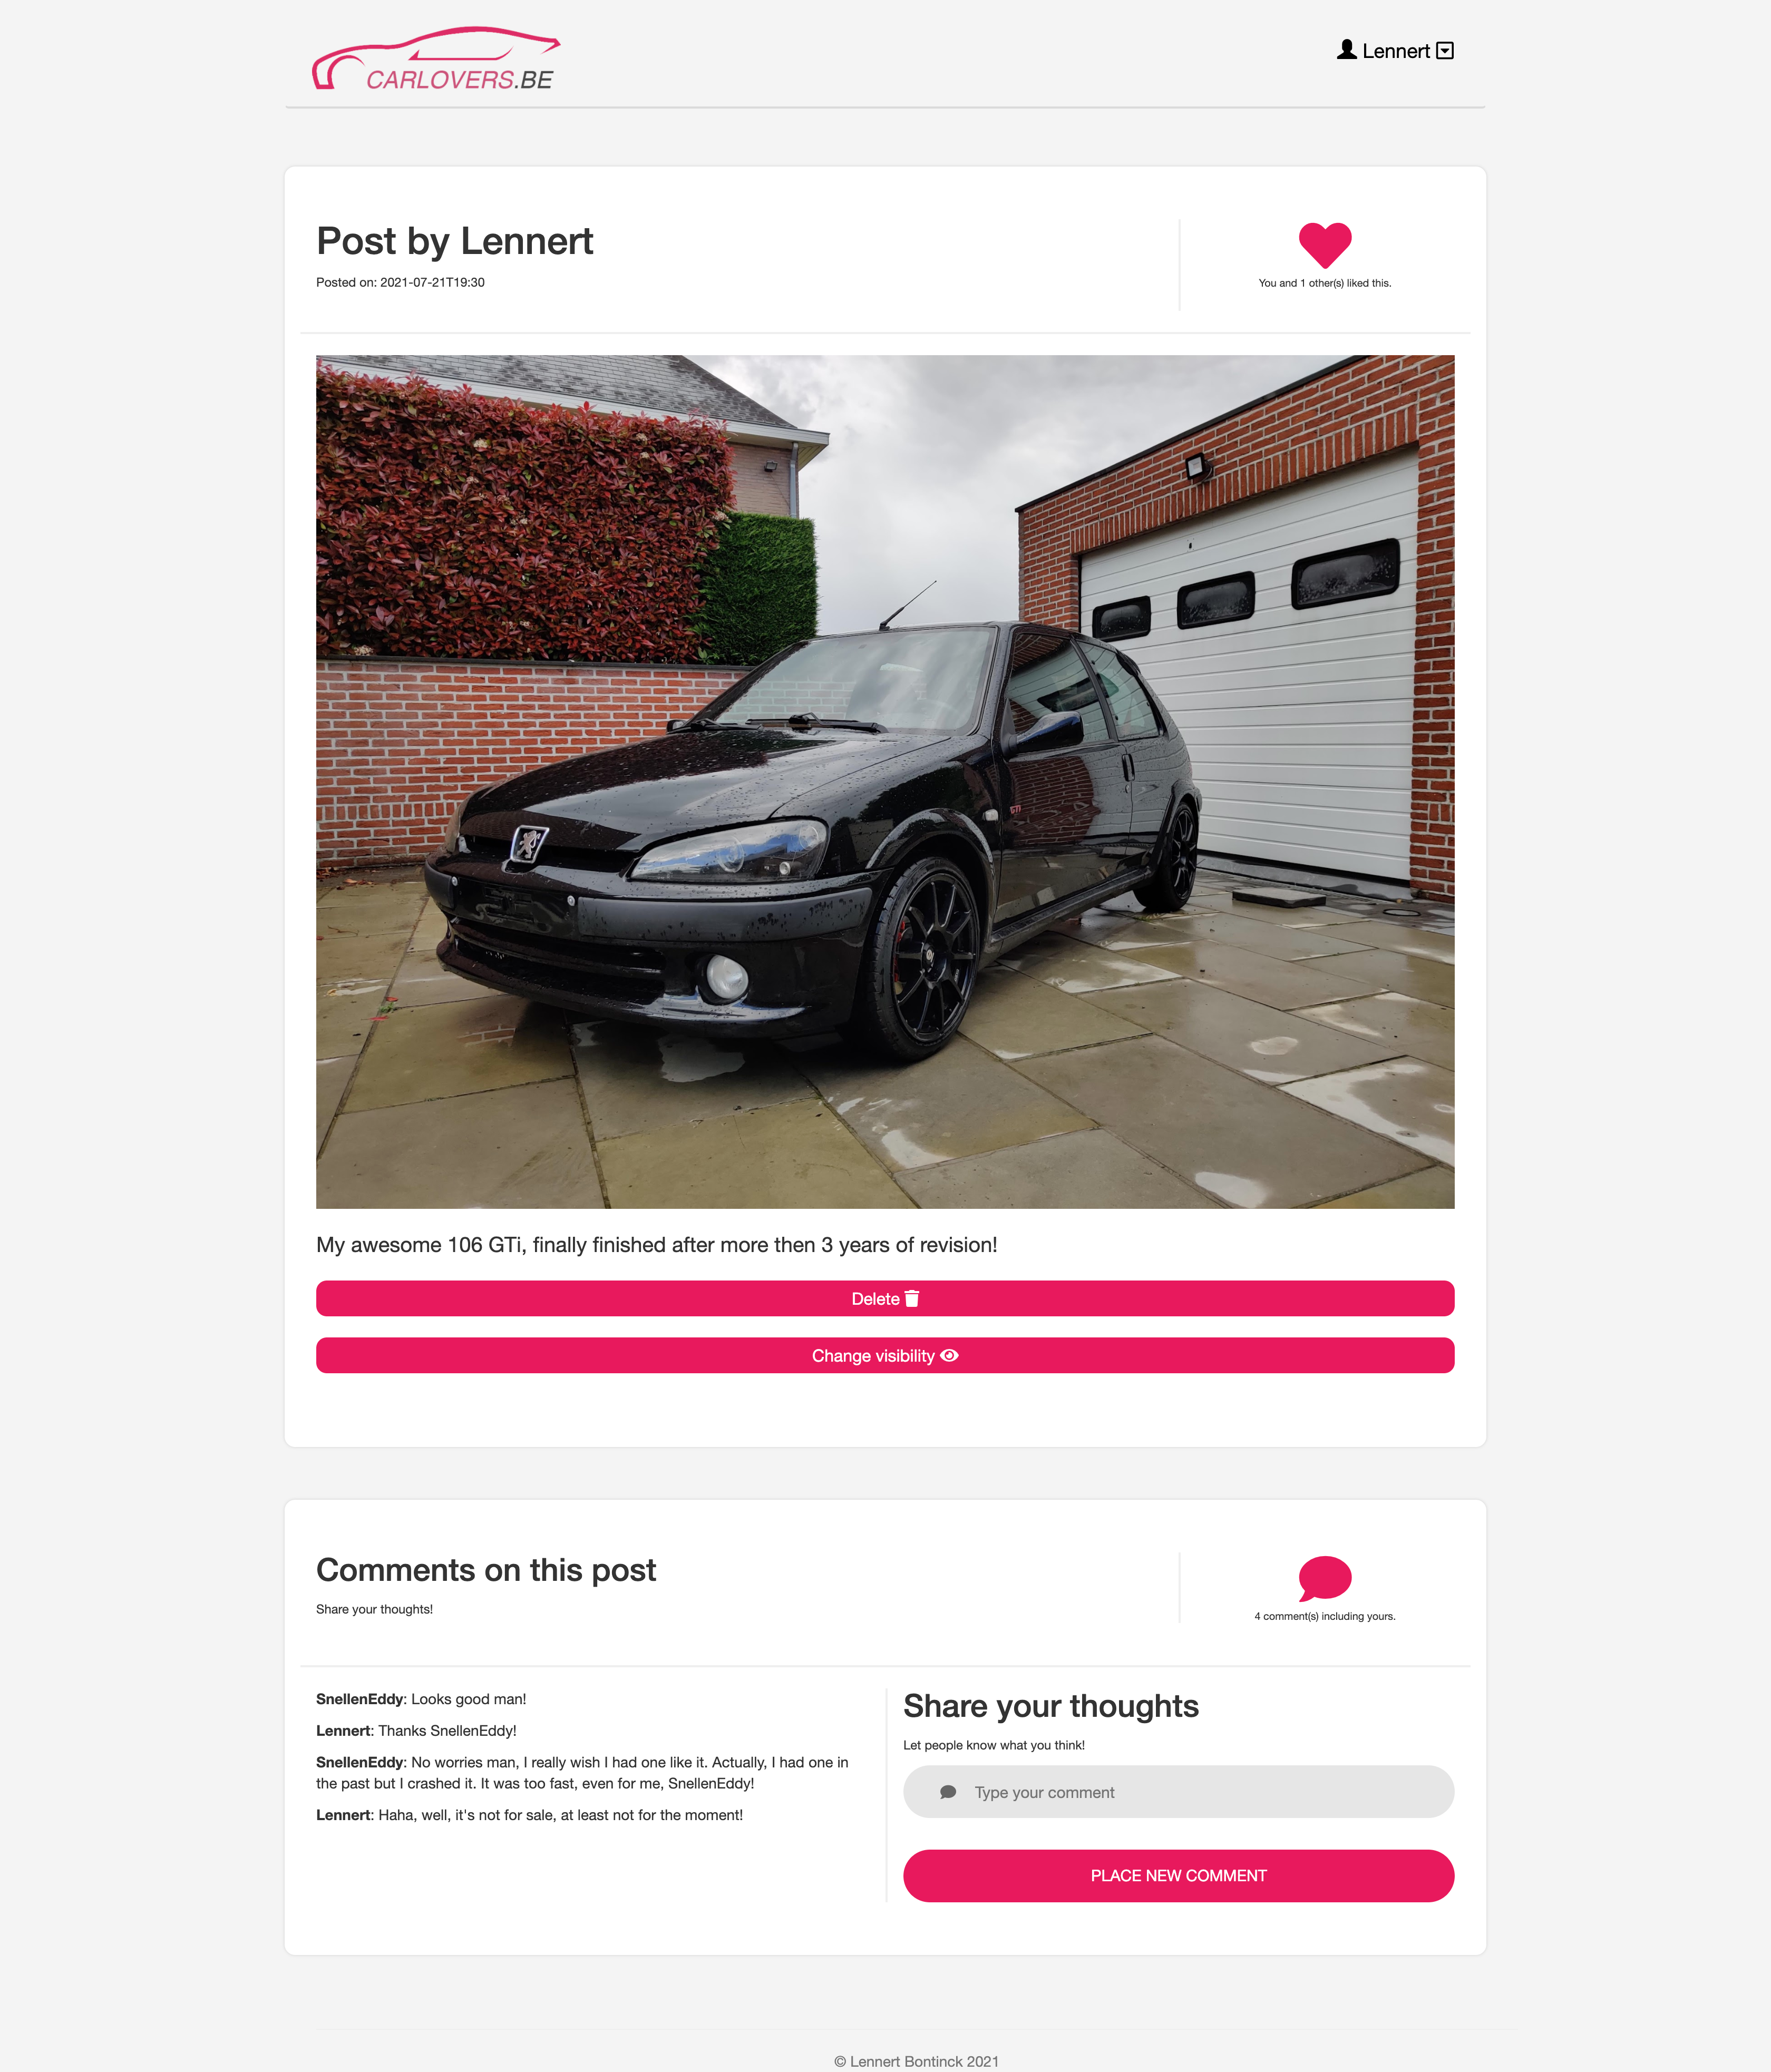
\includegraphics[width=\linewidth]{images/postpage.png}
    \captionsetup{width=0.9\linewidth}
    \captionsetup{justification=centering}
    \caption{The detail page of single post.}
    \label{fig:single}
\end{figure}


\clearpage
\section*{Add post end edit visibility}

\begin{figure}[H]
     \centering
     \begin{subfigure}[b]{0.9\textwidth}
         \centering
         \includegraphics[width=\textwidth]{images/newpost2.png}
         \caption{The add post page.}
         \label{fig:addpost}
     \end{subfigure}
     \hfill
     \begin{subfigure}[b]{0.9\textwidth}
         \centering
         \includegraphics[width=\textwidth]{images/edit.png}
         \caption{The edit visibility page.}
         \label{fig:editpost}
     \end{subfigure}
        \caption{The add post page end edit visibility page for managing posts.}
        \label{fig:postmanage}
\end{figure}


\section*{Limited visibility}

\begin{figure}[H]
     \centering
     \begin{subfigure}[b]{0.9\textwidth}
         \centering
         \includegraphics[width=\textwidth]{images/home.png}
         \caption{Homepage of user who can't see JohnyBravo's post.}
         \label{fig:homenormal}
     \end{subfigure}
     \hfill
     \begin{subfigure}[b]{0.9\textwidth}
         \centering
         \includegraphics[width=\textwidth]{images/homesnellen.png}
         \caption{Homepage of user who can see JohnyBravo's post.}
         \label{fig:homesnellen}
     \end{subfigure}
        \caption{Different posts are shown on the home page for different users according to the visibility settings.}
        \label{fig:homedifferent}
\end{figure}